\section{Introducció i Objectius}
El present treball forma part de l'assignatura de Sistemes de Propulsió d'Aeronaus. Gran part d'aquesta assignatura consisteix en l'estudi dels tipus de motors d'una aeronau i de les possibilitats d'optimització, a més de la parametrització dels motors tant en cas ideal com en cas real.\\
Per tal de duu a terme un estudi més profund de les àrees de coneixement relacionades amb l'assignatura es proposa la realització d'aquest treball. L'objectiu es el disseny preliminar de la motorització d'un avió. Només es donen tres condicions de disseny, de manera que el sistema no queda definit, si no que s'han d'establir certs criteris per a aconseguir tots els paràmetres del motor. En les següents pàgines es discutirà quin tipus de motor pot ser adequat i el criteri de disseny a utilitzar. Seguidament s'implementarà aquest criteri per obtenir alguns dels paràmetres del avió i després es calcularà la resta tenint en compte que el motor es real. Un cop obtinguda la parametrització, s'afegirà al motor un mixer i un postcombustor. En cas que s'hagi decidit afegir un fan, es seleccionarà l'hèlix. Posteriorment, i un cop obtingut els flux màssic tant d'aire com de combustible, es calcularan les àrees del motor.    

Sample Figure
\begin{figure}[H]
	\centering
	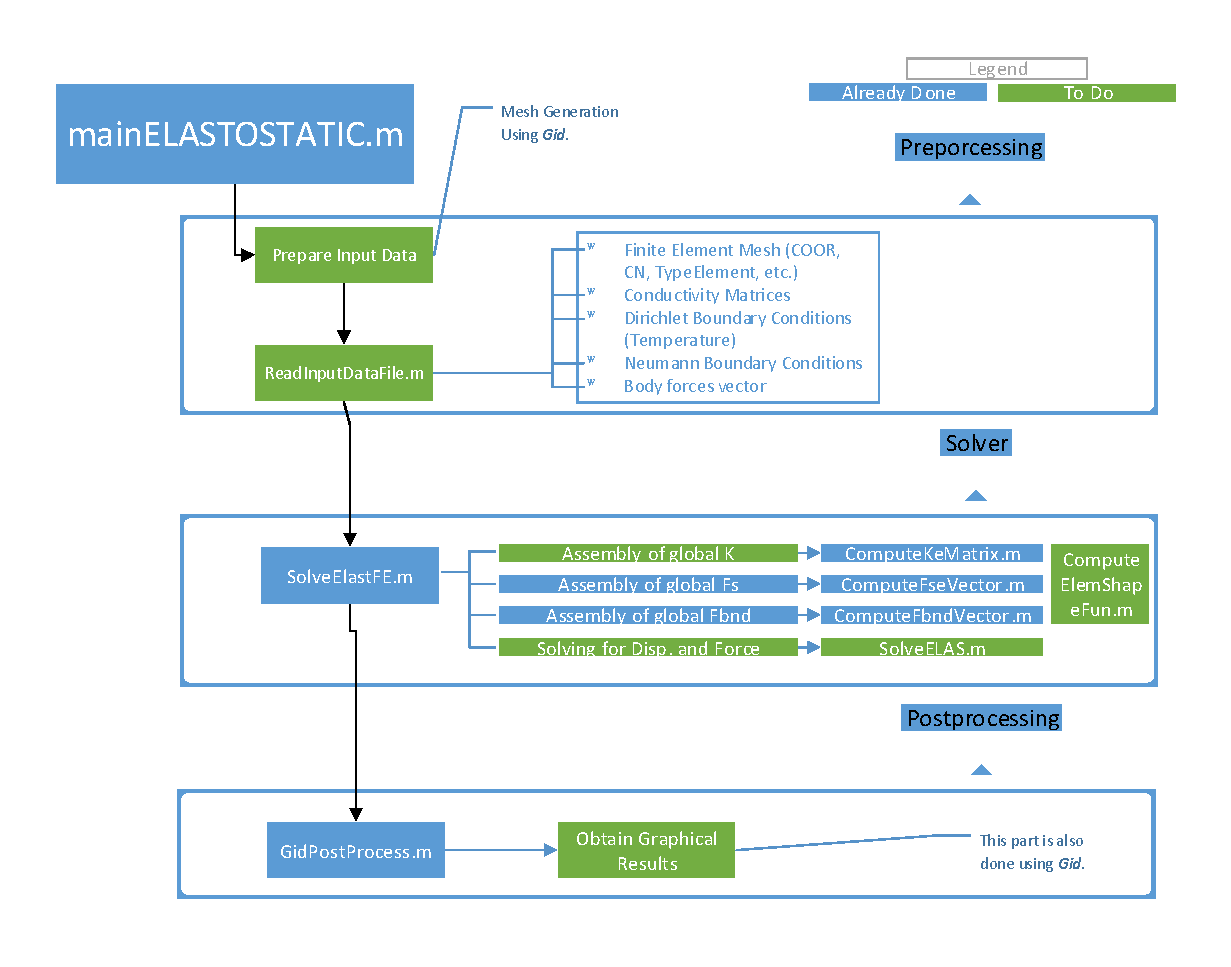
\includegraphics[scale=0.9]{./pics/sample}
	\caption{Sample Caption}
\end{figure}
Numbered equation:
\begin{equation}
	K^e = \sum_{g=1}^{m}w_g (J^eB^{e^T}C B^e)_{\xi=\xi_g}
\end{equation}
In line equation:
final Global stiffness matrix K dimensions will be $n_{sd}n_{pt}\times n_{sd}n_{pt}$.

Sample Listing:
\lstinputlisting[caption={ComputeK.m},label={ComputeK}]{./code/sample.m}